\documentclass[../../deep_learning_notes.tex]{subfiles}
\begin{document}
%%%%%%%%%%%%%%%%%%%%%%%%%%%%%%
\section{Gradients for Common Layers}
%%%%%%%%%%%%%%%%%%%%%%%%%%%%%%
\subsection{Dense Layer}
Let's consider the simplest case of linear transformations using 2-D matrices
\begin{align*}
    Y &= XW + b\\
    X &\in \mathbb{R}^{N \times p}, W \in \mathbb{R}^{p \times k}, Y \in \mathbb{R}^{N \times k}, b \in \mathbb{R}^{k}
\end{align*}
where $N$ is the number of data points, $p$ is the dimension of the input vectors and $k$ is the dimension of output vectors. Instead of calculating the Jacobian, we skip directly to calculation of the gradients, and look at each element of that matrix
\begin{align*}
    \frac{dL}{dW} &= \frac{dL}{dY} \frac{dY}{dW}\\
    \frac{dL}{dW_{ij}} &= \sum_{l=1}^{N} \frac{dL}{dY_{lj}} \frac{dY_{lj}}{dW_{ij}}
\end{align*}
because $W_{ij}$ is used in every example for calculating the $j^{th}$ column of the output matrix. Let's look at the formula for $Y_{lj}$ to get the derivative
\begin{align*}
    Y_{lj} &= X_{l1}W_{1j} + \cdots + X_{li}W_{ij} + \cdots + X_{lp}W_{pj} + b_{j}\\
    \frac{dY_{lj}}{dW_{ij}} &= X_{li}\\
    \implies \frac{dL}{dW_{ij}} &= \sum_{l=1}^{N} \frac{dL}{dY_{lj}} X_{li} = \sum_{l=1}^{N} X^{T}_{il}\frac{dL}{dY_{lj}}\\
    \frac{dL}{dW} &= X^{T} \frac{dL}{dY}
\end{align*}
and consequently, we often loosely denote $dY/dW = X^{T}$, although technically this derivative is a Jacobian matrix of size $N \times k \times p \times k$ which is very difficult to not only compute, but also work with downstream. The error notation to directly work with the gradients comes in handy.\newline

We also need to consider the gradient with input $X$, since that may be used downstream for calculating the gradients in parent layers.
\begin{align*}
    \frac{dL}{dX} &= \frac{dL}{dY} \frac{dY}{dX}\\
    \frac{dL}{dX_{ij}} &= \sum_{l=1}^{k} \frac{dL}{dY_{il}} \frac{dY_{il}}{dX_{ij}}
\end{align*}
since the data point $i$ will only influence the data point $i$ in $Y$. Other data points will not be affected. Further, $X_{ij}$ is used in calculation of every dimension of $Y_{i,:}$. To calculate the gradient,
\begin{align*}
    Y_{il} &= \sum_{t=1}^{p} X_{it}W_{tl}\\
    \frac{dY_{il}}{dX_{ij}} &= W_{jl}\\
    \frac{dL}{dX_{ij}} &= \sum_{l=1}^{k} \frac{dL}{dY_{il}}W_{jl}
    = \sum_{l=1}^{k} \frac{dL}{dY_{il}} W_{lj}^{T}\\
    \implies \frac{dL}{dX} &= \frac{dL}{dY} W^{T}
\end{align*}

Finally, the gradient for the bias term $b$
\begin{align*}
    \frac{dL}{db} &= \frac{dL}{dY} \frac{dY}{db}\\
    \frac{dL}{db_{i}} &= \sum_{l=1}^{N} \frac{dL}{dY_{li}} \frac{dY_{li}}{db}
\end{align*}
since the bias term $b_{i}$ is used in the evaluation of the entire column of $Y$.
\begin{align*}
    \frac{dY_{li}}{db_{i}} &= 1\\
    \frac{dL}{db_{i}} &= \sum_{l=1}^{N} \frac{dL}{dY_{li}}\\
    \frac{dL}{db} &= \bm{1}_{N}\frac{dL}{dY}
\end{align*}
where $\bm{1}_{N} \in \mathbb{R}^{N}$ and all it's elements are ones. This helps do a column wise sum of the gradients of $Y$.

%%%%%%%%%%%%%%%%%%%%%%%%%%%%%%
\subsection{Convolutional Layers}
A very simple demonstration of a convolution operation ($*$) is 
\begin{align*}
    \begin{bmatrix}
        11  &4 &13  &2 &24\\
        5   &1  &7 &21 &20\\
        6  &16 &22 &19  &3\\
       14  &18  &0  &9 &15\\
       10  &12 &23  &8 &17\\
    \end{bmatrix} *
    \begin{bmatrix}
        1 &0 &0\\
        0 &1 &0\\
        0 &0 &1\\
    \end{bmatrix} &= 
    \begin{bmatrix}
        \begin{bmatrix}
            11  &4 &13\\
            5   &1  &7\\
            6  &16 &22
        \end{bmatrix}
        &\begin{bmatrix}
            4 &13  &2\\
            1  &7 &21\\
            16 &22 &19
        \end{bmatrix}
        &\begin{bmatrix}
            13  &2 &24\\
            7 &21 &20\\
            22 &19  &3\\
        \end{bmatrix}\\
        \begin{bmatrix}
            5   &1  &7\\
            6  &16 &22\\
            14  &18 &0
        \end{bmatrix}
        &\begin{bmatrix}
            1  &7 &21\\
            16 &22 &19\\
            18 &0 &9
        \end{bmatrix}
        &\begin{bmatrix}
            7 &21 &20\\
            22 &19  &3\\
            0 &9  &15\\
        \end{bmatrix}\\
        \begin{bmatrix}
            6  &16 &22\\
            14  &18 &0\\
            10  &12 &23
        \end{bmatrix}
        &\begin{bmatrix}
            16 &22 &19\\
            18 &0 &9\\
            12 &23 &8
        \end{bmatrix}
        &\begin{bmatrix}
            22 &19  &3\\
            0 &9  &15\\
            23 &8  &17
        \end{bmatrix}
    \end{bmatrix}.
    \begin{bmatrix}
        1 &0 &0\\
        0 &1 &0\\
        0 &0 &1\\
    \end{bmatrix}\\ &=
    \begin{bmatrix}
        34 &30 &37\\
        21 &32 &41\\
        47 &24 &48\\
    \end{bmatrix}
\end{align*}
The small $3 \times 3$ matrix slides over the entire $5 \times 5$ window (without going outside the boundary) to produce the smaller $3 \times 3$ matrix. This operation is a fundamental building block of Convolutional Neural Networks that uses such convolutional filters to detect edges and other image related features.\newline

There is a third dimension to such filters as well. Our input image is usually of the dimensions Height $\times$ Width $\times$ Channels, where we have 3 channels in an RGB image. When we apply a convolution operation to this, we will also specify the number of such filters to apply. That is, instead of separately applying say $f$ different filters, we use a matrix of 4-D dimensions, where the third dimension is number of imput channels, and fourth dimension is the number of output channels $f$. The output will be of 3 dimensions where the third dimension is of size $f$. This means that we have stacked the outputs of all $f$ filters together to produce a 3D matrix. This multidimensional approach makes the whole process much more simpler and efficient. This concept extends across multiple convolutional layers as well.

A typical convolution operation will work on 4-D tensors
\begin{align*}
    (N \times h_{i} \times w_{i} \times c_{i}) * (f_{1} \times f_{2} \times c_{i} \times c_{o}) \rightarrow (N \times h_{o} \times w_{o} \times c_{o})
\end{align*}
where $N$ is the number of data points, subscript $i$ and $o$ denote input and output, $h$ is height, $w$ is width and $c$ is the number of channels/filters.


%%%%%%%%%%%%%%%%%%%%%%%%%%%%%%
\subsubsection{Single Data Point, Single Filter, Single Channel}
In this simplest case, assume we have an input of shape $h \times w$, a filter of size $f_{1} \times f_{2}$, bias of size $1 \times 1$ (there is one bias term for every filter), and the output is of size $(h - f_{1} + 1) \times (w - f_{2} + 1)$. We assume no strides or padding. Then,
\begin{align*}
    Y &= X * F + b\\
    Y_{ij} &= \begin{bmatrix}
        X_{ij} &\cdots &X_{i(j + f_{2}-1)}\\
        \vdots &\ddots &\vdots\\
        X_{(i+f_{1}-1)j} &\cdots &X_{(i+f_{1}-1)(j+f_{2}-1)}
    \end{bmatrix}*
    \begin{bmatrix}
        F_{11} &\cdots &F_{1f_{2}}\\
        \vdots &\ddots &\vdots\\
        F_{f_{1}1} &\cdots &F_{f_{1}f_{2}}
    \end{bmatrix} + b\\
    &= \sum_{k=1}^{f_{1}} \sum_{l=1}^{f_{2}} F_{kl} X_{(i+k-1)(j+l-1)} + b\\
    \frac{dY_{ij}}{dF_{kl}} &= X_{(i+k-1)(j+l-1)}
\end{align*}
But to calculate the total gradient to $F_{kl}$, we must sum up over all elements of $Y$ since $F_{kl}$ is involved in calculation of each one of them
\begin{align*}
    \frac{dL}{dF_{kl}} &= \sum_{i=1}^{h - f_{1} + 1} \sum_{j=1}^{w - f_{2} + 1} \frac{dL}{dY_{ij}} \frac{dY_{ij}}{dF_{kl}}
    = \sum_{i=1}^{h - f_{1} + 1} \sum_{j=1}^{w - f_{2} + 1} \frac{dL}{dY_{ij}} X_{(i+k-1)(j+l-1)}\\
    &= X_{(k:h-f_{1}+k)(l:w-f_{2}+l)} * \frac{dL}{dY}\\
    \implies \frac{dL}{dF} &= X * \frac{dL}{dY}
\end{align*}
which is a convolution operation between the gradients and input. This is analogous to the dense layer case where we simply multiplied gradients with the matrix $X$. The key take away is that the gradient is being summed over multiple elements of matrix $X$ rather than just a single element.\newline

For $b$, the calculation of gradients is simpler, since $b$ is used in calculation of all elements of $Y$
\begin{align*}
    \frac{dL}{db} &= \sum_{i=1}^{h+f_{1}-1} \sum_{j=1}^{w+f_{2}-1} \frac{dL}{dY_{ij}} \frac{dY_{ij}}{db}\\
    \frac{dY_{ij}}{db} &= 1\\
    \implies \frac{dL}{db} &= \sum_{i=1}^{h+f_{1}-1} \sum_{j=1}^{w+f_{2}-1} \frac{dL}{dY_{ij}}\\
    &= \bm{1}_{h+f_{1}-1}\frac{dL}{dY}\bm{1}_{w+f_{2}-1}
\end{align*}

We may also require the gradients for $X$, in case $X$ itself is the output of some other operation
\begin{align*}
    Y &= X * F + b\\
    Y_{ij} &= \sum_{k=1}^{f_{1}} \sum_{l=1}^{f_{2}} F_{kl} X_{(i+k-1)(j+l-1)} + b\\
\end{align*}
Similar to the gradients for $F$, we sum over all the elements of $Y$ that utilize $X_{kl}$ to get the total gradient at $X_{kl}$. The corner elements of the window of such elements of $Y$ is represented in figure ~\ref{fig:gradient_conv_1}
\begin{figure}[h]
    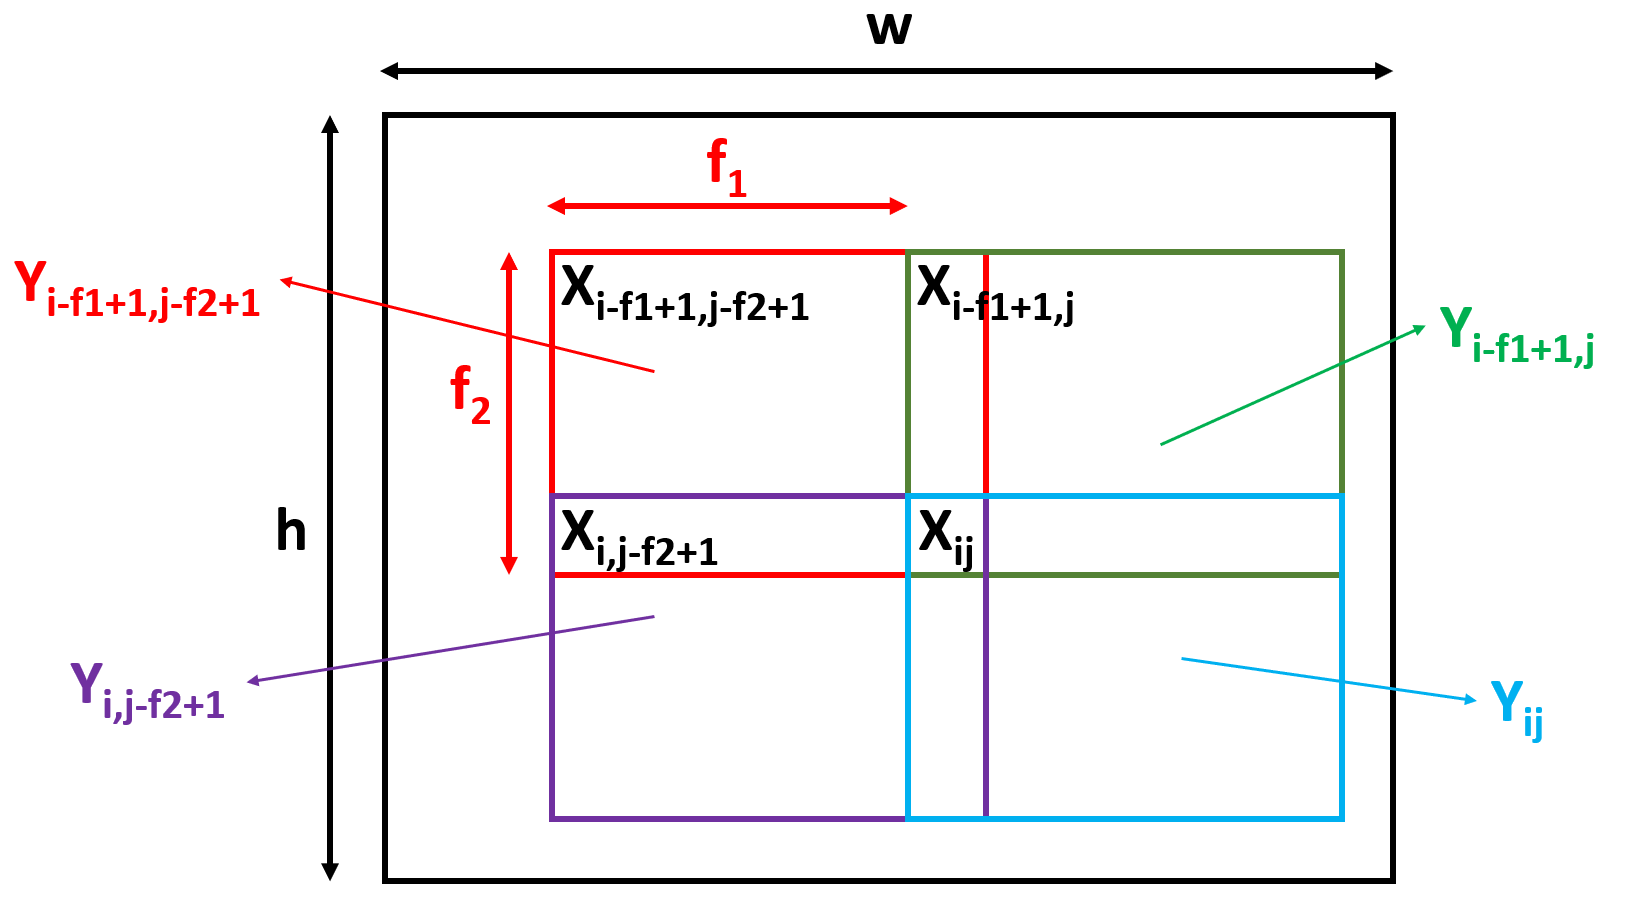
\includegraphics[scale=0.5]{gradient_conv_1}
    \centering
    \caption {The black box represents $X$, while the red, green, purple and sky blue boxes represent the four extreme filters that will contain $X_{ij}$ as a part of their calculation. In all these four filters, $X_{ij}$ will occupy one corner of the filter.}
    \label{fig:gradient_conv_1} %\ref{fig:gradient_conv_1}
\end{figure}
From the figure, we conclude that
\begin{alignat*}{2}
    Y_{(i-f_{1}+1)(j-f_{2}+1)} &= F_{f_{1}f_{2}}X_{ij} &+ \text{other terms}\\
    Y_{(i-f_{1}+1)j} &= F_{f_{1}1}X_{ij} &+ \text{other terms}\\
    Y_{i(j-f_{2}+1)} &= F_{1f_{2}}X_{ij} &+ \text{other terms}\\
    Y_{ij} &= F_{11}X_{ij} &+ \text{other terms}\\
\end{alignat*}
or, the derivative of element of $Y$ will be mapped with the element of the flipped version of $F$, which we denote by $F^{flip}$
\begin{align*}
    F^{flip} &= \begin{bmatrix}
        F_{f_{1}f_{2}} &\cdots &F_{f_{1}1}\\
        \vdots &\ddots &\vdots\\
        F_{1f_{2}} &\cdots &F_{11}\\
    \end{bmatrix}\\
    \frac{dL}{dX_{ij}} &= \sum_{k=f_{1}}^{1} \sum_{l=f_{2}}^{1} \frac{dL}{dY_{(i-k+1)(j-l+1)}} \frac{dY_{(i-k+1)(j-l+1)}}{dX_{ij}}\\
    &= \sum_{k=f_{1}}^{1} \sum_{l=f_{2}}^{1} \frac{dL}{dY_{(i-k+1)(j-l+1)}} F_{kl}
    = \frac{dL}{dY_{(i-f_{1}+1:i)(j-f_{2}+1:j)}} * F^{flip}
\end{align*}
Also, this scheme of finding the corresponding elements of $Y$ for gradients fails near the edges and corners as the index of $Y$ will become negative in some cases. For instance, for $X_{11}$, the left top element of $Y$ for gradient will be $Y_{(2-f_{1})(2-f_{2})}$. This suggests that we need to pad $dL/dY$ with zeros so that the formula developed above is valid even in the corner cases. The horizontal padding is of size $f_{2}-1$ while the vertical is $f_{1}-1$
\begin{align*}
    \frac{dL}{dY^{pad}} =
    \begin{bmatrix}
        0 &\cdots &0 &\cdots &0\\
        0 &\cdots &\frac{dL}{dY} &\cdots &0\\
        0 &\cdots &0 &\cdots &0
    \end{bmatrix} =
     \begin{bmatrix}
        0 &\cdots &0 &\cdots &0 &\cdots &0\\
        0 &\cdots &\frac{dL}{dY_{11}} &\cdots &\frac{dL}{dY_{1(w-f_{2}+1)}} &\cdots &0\\
        \vdots &\vdots &\vdots &\ddots &\vdots &\vdots &\vdots\\
        0 &\cdots &\frac{dL}{dY_{(h-f_{1}+1)1}} &\cdots &\frac{dL}{dY_{(h-f_{1}+1)(w-f_{2}+1)}} &\cdots &0\\
        0 & \cdots &0 &\cdots &0 &\cdots &0\\
    \end{bmatrix}
\end{align*}
Equipped with these new matrices $dL/dY^{pad}$ and $F^{flip}$, we can write the gradients as
\begin{align*}
    \frac{dL}{dX} &= \frac{dL}{dY^{pad}} * F^{flip}\\
    \frac{dL}{dX} &\in \mathbb{R}^{h \times w}, F^{flip} \in \mathbb{R}^{f_{1} \times f_{2}}\\
    \frac{dL}{dY^{pad}} &\in \mathbb{R}^{((h-f_{1}+1)+2(f_{1}-1) \times (w-f_{2}+1) + 2(f_{2}-1)} \sim \mathbb{R}^{(h+f_{1}-1) \times (w+f_{2}-1)}
\end{align*}
and dimensions check out because
\begin{align*}
    (h+f_{1}-1) - f_{1} + 1 &= h\\
    (w+f_{2}-1) - f_{2} + 1 &= w
\end{align*}
We can also verify that the first two elements of $dL/dX$ are as expected
\begin{align*}
    \frac{dL}{dX_{11}} &= \frac{dL}{dY^{pad}_{11}} F^{Flip}_{f_{1}f_{2}} = \frac{dL}{dY_{11}} F_{11}\\
    \frac{dL}{dX_{12}} &= \frac{dL}{dY^{pad}_{11}} F^{Flip}_{f_{1}(f_{2}-1)} + \frac{dL}{dY^{pad}_{12}} F^{Flip}_{f_{1}f_{2}}\\ &= \frac{dL}{dY_{11}} F_{12} + \frac{dL}{dY_{12}} F_{11}\\
\end{align*}

Summarizing,
\begin{align*}
    Y &= X * F + b\\
    \frac{dL}{dF} &= X * \frac{dL}{dY}\\
    \frac{dL}{db} &= \bm{1}_{h+f_{1}-1}\frac{dL}{dY}\bm{1}_{w+f_{2}-1}\\
    \frac{dL}{dX} &= \frac{dL}{dY^{pad}} * F^{flip}
\end{align*}


\subsubsection{Single Data Point, Single Filter, Multiple Channels}
Assume we have an input of shape $h \times w \times d$, a filter of size $f_{1} \times f_{2} \times d$, bias of size $1 \times 1$, and the output is of size $(h - f_{1} + 1) \times (w - f_{2} + 1)$. We assume no strides or padding. Then,
\begin{align*}
    Y &= X * F + b\\
\end{align*}

The case is similar to the previous case, but instead of a 2D filter, we are now working in 3D. The formulae will remain the same, since the convolution operator will still be sliding on the 2D plane of height $\times$ width
\begin{align*}
    \frac{dL}{dF} &= X * \frac{dL}{dY}\\
    \frac{dL}{db} &= \bm{1}_{h+f_{1}-1}\frac{dL}{dY}\bm{1}_{w+f_{2}-1}\\
    \frac{dL}{dX} &= \frac{dL}{dY^{pad}} * F^{flip}
\end{align*}

where $Y^{pad}$ only has padding in the height and width dimensions. Similarly, $F^{flip}$ flips each 2D plane individually, there is no transformation along the depth.


%%%%%%%%%%%%%%%%%%%%%%%%%%%%%%
\subsection{Max Pooling 2D Layer}
MaxPooling is an operation that operates on windows similar to convolutional filters. This layer gives a single output that is the maximum of all the inputs in the given window.
\begin{align*}
    MaxPool2D \bigg( \begin{bmatrix}
        11  &4 &13  &2\\
        5   &1  &7 &21\\
        6  &16 &22 &19\\
       14  &18  &0  &9
    \end{bmatrix}, 2 \times 2, stride = 1 \bigg) &=
    \begin{bmatrix}
        11  &13 &21\\
        16  &22 &22\\
        18  &22 &22\\
    \end{bmatrix}\\
    MaxPool2D \bigg( \begin{bmatrix}
        11  &4 &13  &2\\
        5   &1  &7 &21\\
        6  &16 &22 &19\\
       14  &18  &0  &9
    \end{bmatrix}, 2 \times 2, stride = 2 \bigg) &=
    \begin{bmatrix}
        11 &21\\
        18 &22\\
    \end{bmatrix}\\
\end{align*}
We usually use this layer with strides $=$ size of layer, with the same height and width. The large strides allow rapid shrinkage of the input to smaller size so that the number of connections with a dense layer downstream are low.\newline

This layer is useful so that the model is invariant to any rotation of the input. Suppose we have a $2 \times 2$ sized filter, and the maximum value is say $3$. The layer will give the same output irrespective of in which of the $4$ cells $3$ is present. Thus, pooling layer helps preserve the core information even when the image may be shifted, rotated etc.\newline

The size of output is determined in the same manner as convolutional layers. The layer will operate on each channel individually, causing no change in number of channels from input to output. Thus, the only dimensions that change are width and height.\newline

Max function has no learnable parameters, and thus only acts as gateway for redirecting flow of gradients. The gradient will only flow through the cell actually used in computation of the max (the maximum valued cell) since adjusting the other cells by little amounts will not change the output.\newline
In case multiple cells satisfy the maximum condition (discontinuity), there is no single way to distribute the gradient. Usually, the first entry corresponding to the maximum has the gradient flow. When weights are initialized properly, this problem will be rare.
\begin{align*}
    X &= \begin{bmatrix} 1 &0\\ 2 &0\\\end{bmatrix}\\
    Y &= MaxPool2D(X) = 2, \; Y_{max} = (2,1)\\
    \frac{dL}{dX} &= \frac{dL}{dY}\frac{dY}{dX}
    = \begin{bmatrix} 0 &0\\ \frac{dL}{dY} &0\\\end{bmatrix}
\end{align*}

When implementing this layer, we will remember the index of the input where the maximum occurred and allow gradient flow only through that cell. In case the same input cell is used in multiple max (stride $=$ 1 for instance), the total gradient gets added up
\begin{align*}
    X &= \begin{bmatrix} 1 &0 &1\\ 2 &0 &1\\ 0 &1 &0\end{bmatrix}\\
    Y &= MaxPool2D(X) = \begin{bmatrix} 2 &1\\ 2 &1\end{bmatrix}, \; Y_{max} = \begin{bmatrix} 2,1 &1,3\\ 2,1 &2,3\end{bmatrix}\\
    \frac{dL}{dX} &= \frac{dL}{dY}\frac{dY}{dX}
    = \begin{bmatrix}[1.5] 0 &0 &\frac{dL}{dY_{12}}\\ \frac{dL}{dY_{11}} + \frac{dL}{dY_{21}} &0 &\frac{dL}{dY_{22}}\\ 0 &0 &0\end{bmatrix}
\end{align*}


%%%%%%%%%%%%%%%%%%%%%%%%%%%%%%
\subsection{Flatten Layer}
Similar to MaxPool, this layer has no learnable parameters and just restructres the input data into a flat 1D array. The gradient flow is simply remembering which index in the original tensor corresponds to the considered index in the 1D array. The total number of elements in the input and output remain the same.
\end{document}